\section*{Arrival Functions}
Three models are considered in this section, a staircase, an affine, and a linear model as seen on \autoref{fig:arrivalCurves}. The staircase and affine models are used to approximate the real unknown arrival function, while the linear model is a service curve showing the capabilities of the network.\\

The staircase arrival model in relation to the real unknown arrival function is given by
\begin{flalign}
  R(t) \leq Sc(t) &= \left\lceil \frac{t - \mathrm{offset}}{T} \right\rceil \times P \ \ ,&
\end{flalign}
%
\begin{where}
  \va{R(t)}{is the real unknown arrival curve.}{}
  \va{Sc(t)}{is the staircase model arrival curve for the wheel sensor data.}{}
  \va{t}{is the time.}{}
  \va{\mathrm{offset}}{is the time offset measured from $t = 0$ to first packet arrival.}{}
  \va{T}{is the period time for packet arrivals.}{}
  \va{P}{is the packet size.}{}
\end{where}

The worst case is when the offset goes to zero, this means that a packet arrives at time zero.

\begin{figure}[H]
  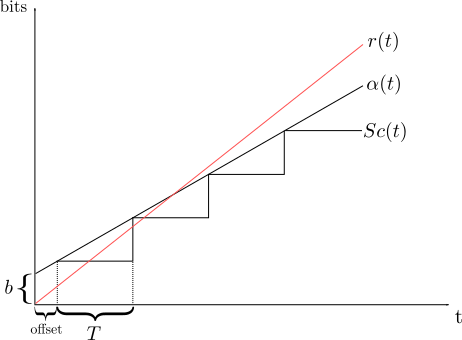
\includegraphics[width = .4\textwidth]{arrivalCurves}
  \caption{$Sc(t)$ is the staircase arrival curve, $\alpha(t)$ is the affine model arrival curve and $r(t)$ is the service curve defined by the capabilities of the CAN Bus.}
  \label{fig:arrivalCurves}
\end{figure}

The affine arrival model in relation to the real unknown arrival function is given by
\begin{flalign}
  R(t) \leq \alpha (t) &= b + \frac{P}{T} t &
\end{flalign}
%
\begin{where}
  \va{\alpha}{is the affine model arrival curve}{}
  \va{b}{is the crossing of the affine curve with the y-axis}{}
\end{where}
%
The relation between both models and the unknown real arrival function is then given by
\begin{flalign}
  R &\leq Sc \leq \alpha &
\end{flalign}

\subsection{Wheel Sensor Data Arrival}
The staircase arrival model for the wheel sensor data is
\begin{flalign}
  Sc_\mathrm{w} (t) &= \left\lceil \frac{t - \cancelto{0}{\mathrm{offset}} \ \ \ }{T_\mathrm{w}} \right\rceil \times P_\mathrm{w}& \\
  Sc_\mathrm{w} (t) &= \left\lceil \frac{t}{0.04} \right\rceil \times 160 \ \ ,&
\end{flalign}
where $P_\mathrm{w} = 20\times 8$ since the packet size is \SI{20}{B}, which means that \SI{160}{b} arrive at each time interval, $T = 0.04$. The time offset is set to zero in order to model for worst case.
%
%\begin{where}
%  \va{Sc_\mathrm{w} (t)}{is the staircase model arrival curve for the wheel sensor data.}{}
%  \va{t}{is the time.}{}
%  \va{\mathrm{offset}}{is the time offset measured from $t = 0$ to first packet arrival.}{}
%  \va{T_\mathrm{w}}{is the period time for packet arrivals from the wheel sensors.}{}
%  \va{P_\mathrm{w}}{is the packet size containing the wheel sensor data.}{}
%\end{where}
%
%
The affine arrival model for the wheel sensor data is
\begin{flalign}
  \alpha_\mathrm{w} (t) &= b + \frac{P_\mathrm{w}}{T_\mathrm{w}} t & \\
  \alpha_\mathrm{w} (t) &= 160 + \frac{160}{0.04} t  = 160 + 6.4 t \ \ ,&
\end{flalign}
where $b = P_\mathrm{w} = 160$ since the time offset is set to zero to model worst case.
%
%\begin{where}
%  \va{\alpha_\mathrm{w} (t)}{is the affine model arrival curve for the wheel sensor data}{}
%  \va{b}{is the crossing of the affine curve with the y-axis}{}
%\end{where}
%
%
\subsection{Electronic Speed Control (ESC) Data Arrival}
The staircase arrival model for the wheel sensor data is
\begin{flalign}
  Sc_\mathrm{ESC} (t) &= \left\lceil \frac{t - \cancelto{0}{\mathrm{offset}} \ \ \ }{T_\mathrm{ESC}} \right\rceil \times P_\mathrm{ESC}& \\
  Sc_\mathrm{ESC} (t) &= \left\lceil \frac{t}{0.4} \right\rceil \times 64 \ \ ,&
\end{flalign}
where $P_\mathrm{ESC} = 8\times 8$ since the packet size is \SI{8}{B}, which means that \SI{64}{b} arrive at each time interval, $T = 0.4$. The time offset is again set to zero in order to model for worst case.
%
%\begin{where}
%  \va{Sc_\mathrm{w} (t)}{is the staircase model arrival curve for the wheel sensor data.}{}
%  \va{t}{is the time.}{}
%  \va{\mathrm{offset}}{is the time offset measured from $t = 0$ to first packet arrival.}{}
%  \va{T_\mathrm{w}}{is the period time for packet arrivals from the wheel sensors.}{}
%  \va{P_\mathrm{w}}{is the packet size containing the wheel sensor data.}{}
%\end{where}
%
The affine arrival model for the wheel sensor data is
\begin{flalign}
  \alpha_\mathrm{ESC} (t) &= b + \frac{P_\mathrm{ESC}}{T_\mathrm{ESC}} t & \\
  \alpha_\mathrm{ESC} (t) &= 64 + \frac{64}{0.4} t = 64 + 25.6 t \ \ ,&
\end{flalign}
where $b = P_\mathrm{ESC} = 64$ since the time offset is set to zero to model worst case.

\subsection{Service Model}
The curve for the service model, $r(t)$, is seen in \autoref{fig:arrivalCurves}. The model is linear and defined by the capabilities of the CAN Bus with a rate of \SI{1}{Mbps}.


\section{Token Filter}

\begin{figure}[H]
  \includegraphics[width = .4\textwidth]{tokenFilter}
  \caption{Token filter}
  \label{fig:tokenFilter}
\end{figure}



%\begin{where}
%  \va{}{}{}
%  \va{}{}{}
%  \va{}{}{}
%  \va{}{}{}
%  \va{}{}{}
%\end{where}
%%






%r(t) is the service curve







